\documentclass[svgnames]{beamer}[10]
\usepackage{pgf}
% \usepackage{babel}
\usepackage[utf8]{inputenc}
\usepackage{beamerthemesplit}
\usepackage{epsfig, subfigure}
\usepackage{graphicx} % Required for including images
\usepackage{url}
\usepackage{srcltx}
\usepackage{hyperref}
\usepackage{tikz}
\usepackage{array}
\usepackage{soul}
\usepackage{natbib}
\usepackage{pgfplots,pgfplotstable}

\definecolor{lightblue}{rgb}{.90,.95,1}
\sethlcolor{lightblue}
\renewcommand<>{\hl}[1]{\only#2{\beameroriginal{\hl}}{#1}}
\definecolor{kugreen}{RGB}{50,93,61}
\definecolor{kugreenlys}{RGB}{132,158,139}
\definecolor{kugreenlyslys}{RGB}{173,190,177}
\definecolor{kugreenlyslyslys}{RGB}{214,223,216}
\definecolor{ku}{RGB}{144,26,30}
\definecolor{ku-yellow}{RGB}{255,249,25}
\setbeamercovered{transparent}
\mode<presentation>
\usetheme[numbers,compress,sidebarshades]{PaloAlto}
\setbeamertemplate{footline}[frame number]

\usepackage{pgfpages}
\usepackage{apalike}
\usepackage{graphicx} % Required for including images
\graphicspath{{figures/}} % Location of the graphics files
\usepackage{booktabs} % Top and bottom rules for table
\usepackage[font=small,labelfont=bf]{caption} % Required for specifying captions to tables and figures
\usepackage{wrapfig} % Allows wrapping text around tables and figures
\usepackage{lipsum,adjustbox}
\usepackage[absolute,overlay]{textpos}
\usepackage{url}
\usepackage{lmodern}
\usepackage{amsmath}
\usepackage{amsfonts}
\usepackage{color}
\usepackage{array}
\usepackage{multirow}
\usepackage{multicol}
\usepackage{rotating}
\usepackage{tikz,pgfplots,pgfplotstable}
\usepackage{tikz-dependency}
\usetikzlibrary{arrows.meta,graphs,graphs.standard,graphdrawing,quotes,shapes}
\usegdlibrary{layered,trees}
\setbeamertemplate{sidebar left}{}
\tikzset{
  invisible/.style={opacity=0},
  visible on/.style={alt={#1{}{invisible}}},
  alt/.code args={<#1>#2#3}{%
    \alt<#1>{\pgfkeysalso{#2}}{\pgfkeysalso{#3}} % \pgfkeysalso doesn't change the path
  },
}
\captionsetup{labelformat=empty}

\makeatletter
\pgfdeclareshape{vector}{
	  \inheritsavedanchors[from={rectangle}]
	  \inheritbackgroundpath[from={rectangle}]
	  \inheritanchorborder[from={rectangle}]
	  \foreach \x in {center,north east,north west,north,south,south east,south west,east,west}{
	    \inheritanchor[from={rectangle}]{\x}
	  }

    \backgroundpath{
      \pgftransformshift{\pgfpoint{-16pt}{-4pt}}
		  \draw[rounded corners=2pt] (0,0) rectangle (32pt,8pt);
    }

    \beforebackgroundpath{
      \draw[step=8pt,help lines,-] (8pt,.1pt) grid (24pt,7.9pt);
    }
}
\makeatother

  \usecolortheme[named=kugreen]{structure}
  \useinnertheme{circles}
  \usefonttheme[onlymath]{serif}
  \setbeamercovered{transparent}
  \setbeamertemplate{blocks}[rounded][shadow=true]
  
\makeatletter
\newcommand\SoulColor{%
  \let\set@color\beamerorig@set@color
  \let\reset@color\beamerorig@reset@color}
\makeatother
\SoulColor

% Outline slides
\AtBeginSection[]
{\begin{frame} \frametitle{Outline} \tableofcontents[currentsection,currentsubsection] \end{frame}}

% \logo{\includegraphics[width=0.8cm]{KULogo}}
%\useoutertheme{infolines} 
\title{Universal Conceptual Cognitive Annotation}
\subtitle{Cross-lingual Semantic Representation for NLP with UCCA}
\author{\bfseries
  Omri Abend$^{*}$ \quad
  Dotan Dvir$^{*}$ \\
  Daniel Hershcovich$^{**}$ \quad
  Jakob Prange$^{***}$ \\
  Nathan Schneider$^{***}$}
\institute{$^{*}$Hebrew University of Jerusalem 
\\ $^{**}$University of Copenhagen
\\ $^{***}$Georgetown University}
\date{Tutorial at COLING 2020 \\
December 12, 2020}

\begin{document}
\frame{\titlepage}

\section{Bird's Eye View}

\begin{frame}{UCCA}
    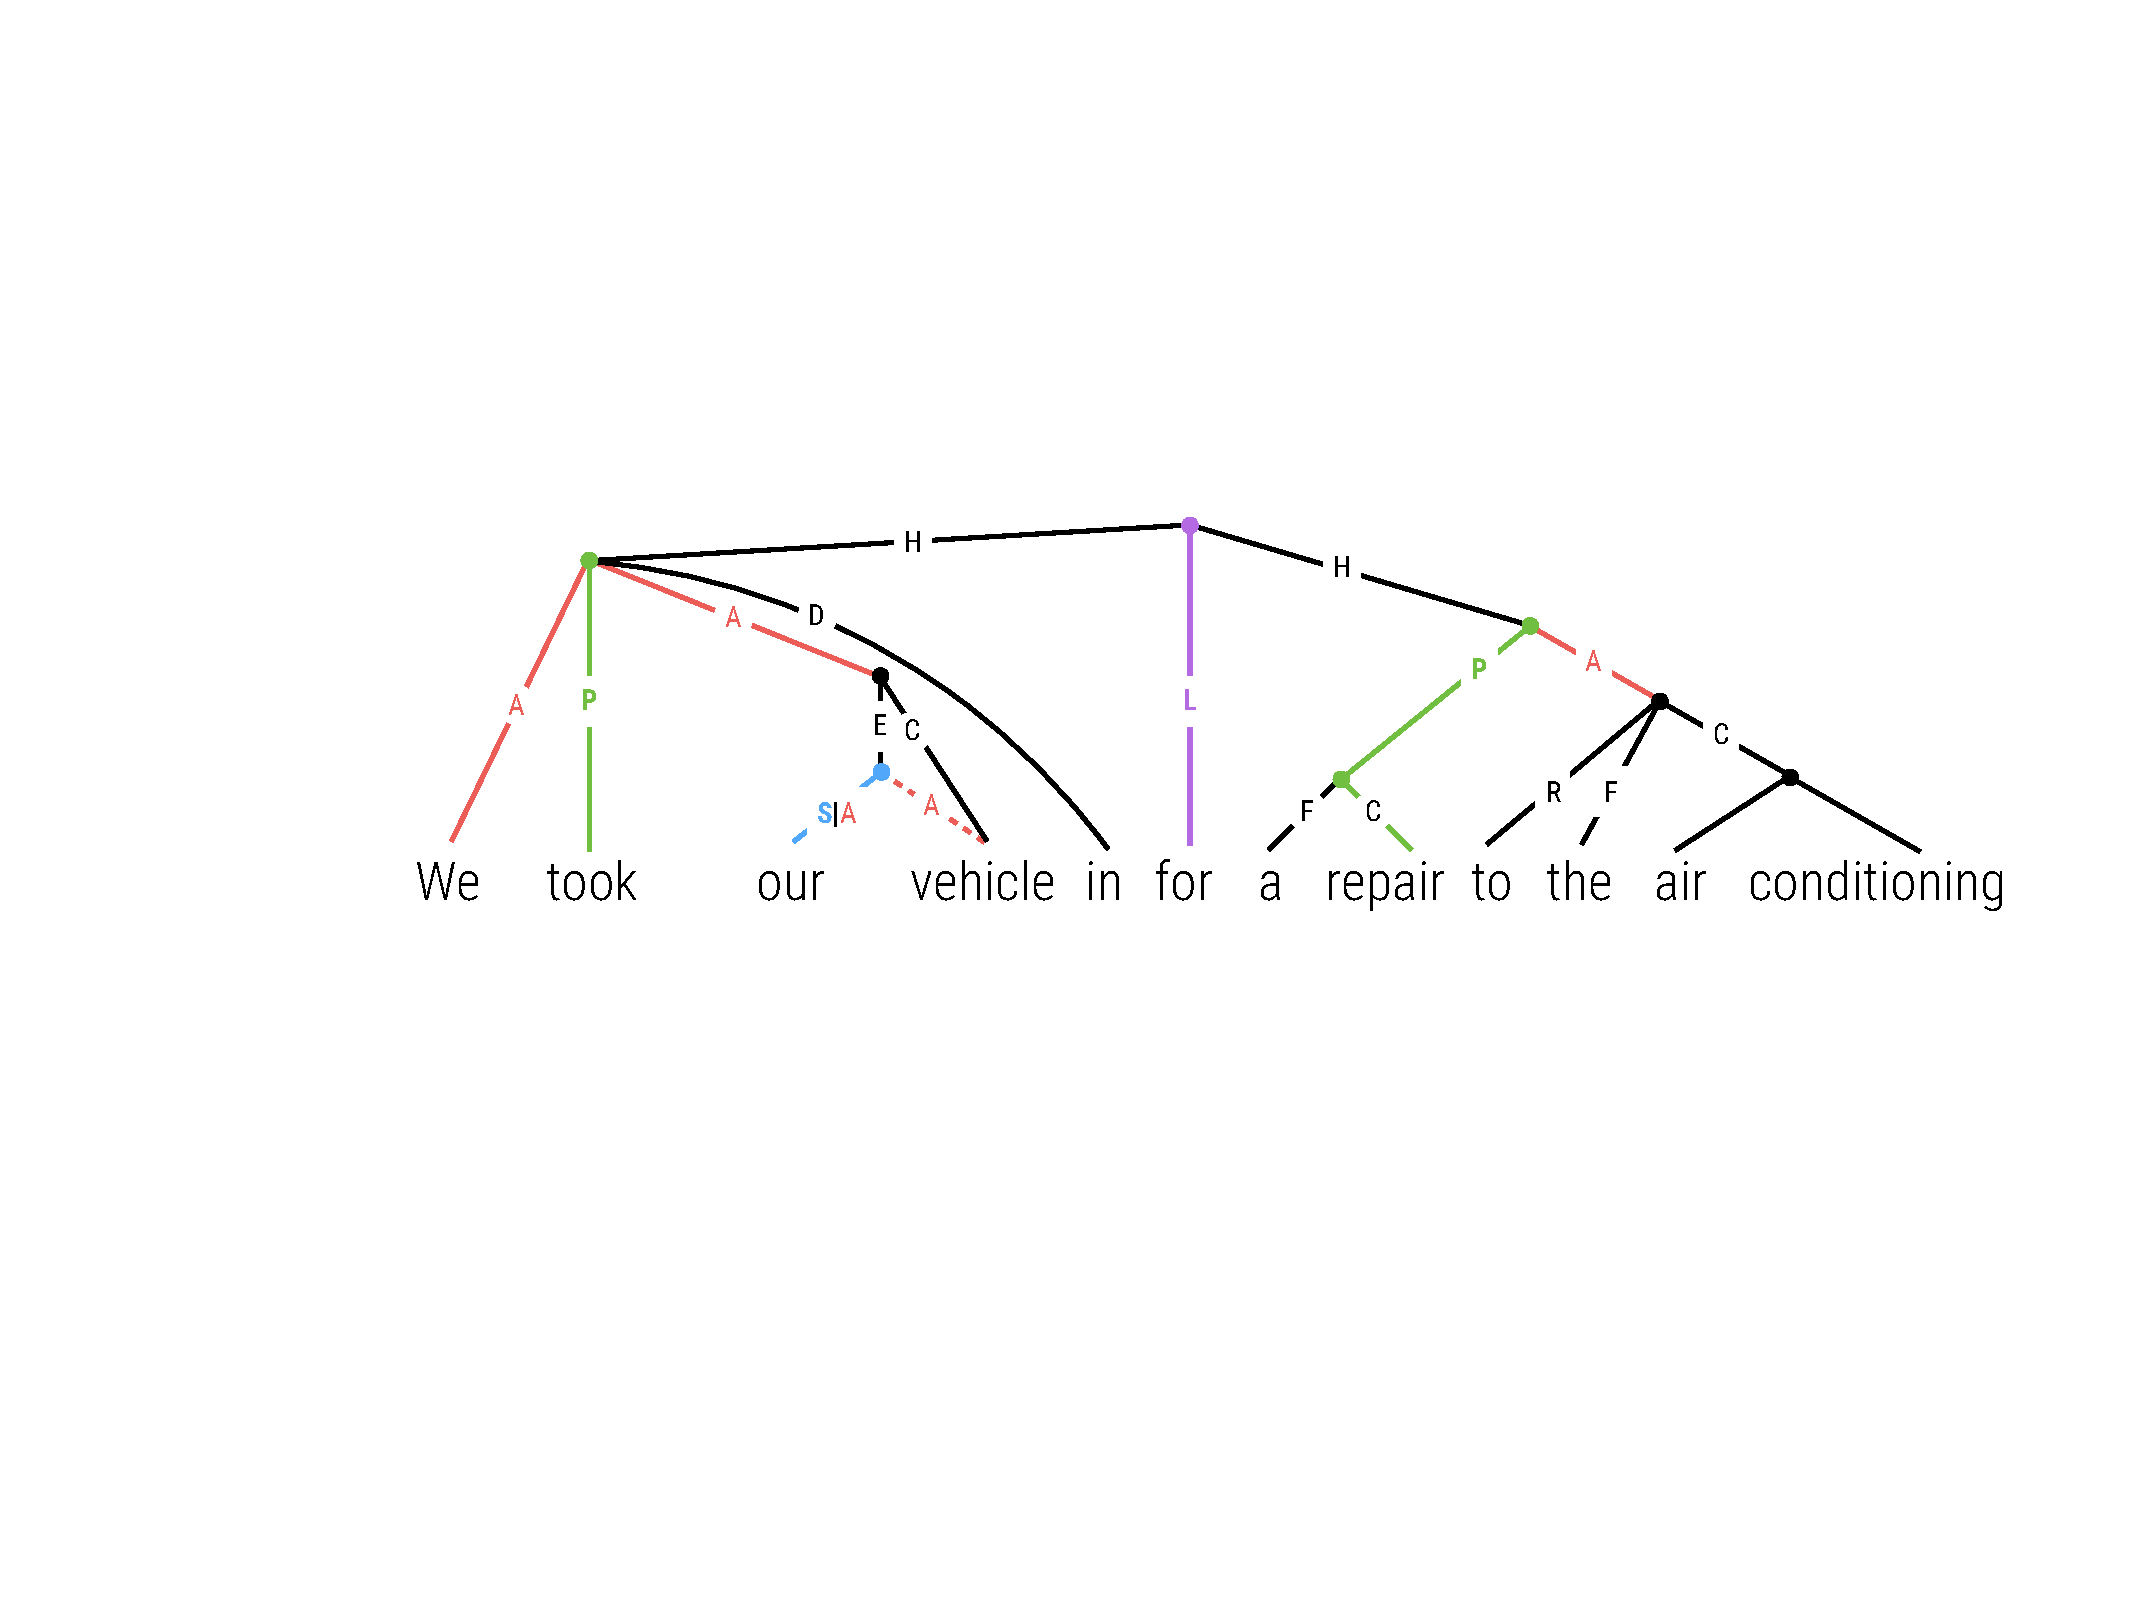
\includegraphics[width=\textwidth]{ex-ucca.pdf}
\end{frame}

\section{Guidelines}

\section{Data}

\section{Extensions}

\begin{frame}
\frametitle{Extensions}
    \begin{itemize}
        \item ``UCCA is built as a multi-layered structure, which allows for its open-ended extension.'' \citep{abend2013universal}
        \item Foundational layer has relatively flat structure, makes coarse distinctions
        \item Additional layers can capture additional semantic phenomena by...
        \begin{itemize}
            \item refining existing categories
            \item introducing new distinctions
            \item adding deeper\slash more complex structure
        \end{itemize}
    \end{itemize}
\end{frame}

\begin{frame}
\frametitle{Extensions: Semantic Roles}
    \begin{itemize}
        \item Labeling all participants as `Participant' does not answer the classic `WDWTW?' (Who did what to whom?)
        \item We need semantic (thematic, theta) roles: \{Agent, Theme, Experiencer, ...\}
        \item Option 1: Refine all Participants with a semantic role
        \item Option 2: Annotate all semantic roles explicitly marked with a lexical item
    \end{itemize}
\end{frame}

\begin{frame}
\frametitle{Extensions: Semantic Roles}
    \begin{itemize}
        \item Option 1: Refine all Participants with a semantic role
        \item \citet{shalev-etal-2019-preparing}
        \item ... (summarize process and findings)
    \end{itemize}
\end{frame}

\begin{frame}
\frametitle{Extensions: Semantic Roles}
    \begin{itemize}
        \item Option 2: Annotate all semantic roles explicitly marked with a lexical item
        \item \citet{prange2019made}
        \item ... (summarize process and findings, including but not focusing on ML experiments)
    \end{itemize}
\end{frame}

\begin{frame}
\frametitle{Extensions: Coreference}
    \begin{itemize}
        \item \citet{prange2019semantically}
        \item ... (tell story from UCCA perspective)
        \item ... (in the end mention comparative experiments with GUM, RED, and OntoNotes. can nicely segue into next section?)
    \end{itemize}
\end{frame}

\section{Comparison to Other Frameworks}
\begin{frame}
\frametitle{Comparison to Other Frameworks}
    \begin{itemize}
        \item Dimensions along which to compare
        \begin{itemize}
            \item \citet{koller2019graph} and \citet{prange2019semantically} taxonomies
            \item theoretical foundations
            \item formal properties
            \item aims, applications, extensions
        \end{itemize}
    \end{itemize}
\end{frame}

\begin{frame}
\frametitle{Comparison to Other Frameworks: AMR}
    \begin{itemize}
        \item ...
    \end{itemize}
\end{frame}

\begin{frame}
\frametitle{Comparison to Other Frameworks: Syntactic Representation}
    \begin{itemize}
        \item ...
    \end{itemize}
\end{frame}

\begin{frame}
\frametitle{Comparison to Other Frameworks: Discourse Representation}
    \begin{itemize}
        \item ...
    \end{itemize}
\end{frame}

\begin{frame}
\frametitle{Comparison to Other Frameworks: MRP Shared Task}
    \begin{itemize}
        \item introduce goals, tools, and findings of MRP shared task
        \item coarsely compare UCCA with PTG, EDS, DRG
    \end{itemize}
\end{frame}

\section{Parsing}


\begin{frame}
\frametitle{UCCA Parsing}
{\Large \textbf{The Task:} Given plain text,
predict its UCCA graph representation.}

\vfill

\begin{center}
    {\rmfamily\small They thought about taking a short break}
\[\Downarrow\]
\scalebox{.5}{
\begin{tikzpicture}[level distance=16mm, sibling distance=28mm, ->, thick,
  level 2/.style={sibling distance=12mm},
  level 3/.style={sibling distance=18mm},
  edge from parent/.append style={nodes={font=\scriptsize}}]
  \tikzstyle{word} = [font=\rmfamily,color=black]
    \node (ROOT) [fill=blue, circle] {}
      child {node (They) [word] {They} edge from parent node[left] {A}}
      child {node [word] {thought} edge from parent node[left] {P}}
      child {node (abouttakingashortbreak) [fill=blue, circle] {}
      {
        child {node [word] {about} edge from parent node[left] {R}}
        child {node (takingabreak) [fill=blue, circle] {}
        {
          child {node [word] {taking} edge from parent node[above] {F}}
          child {node [word] {a} edge from parent node[right] {F}}
          child {node [word] (short) {short} edge from parent[draw=none]}
          child {node [word] {break} edge from parent node[right] {C}}
        } edge from parent node[right] {P} }
      } edge from parent node[right] {A} }
      ;
    \draw[bend left,dashed,->] (abouttakingashortbreak) to node [auto] {\scriptsize A} (They);
    \draw[bend left,->] (abouttakingashortbreak) to node [auto] {\scriptsize D} (short);
\end{tikzpicture}}
\end{center}
\end{frame}

\begin{frame}
\frametitle{Graph Structure}
Labeled directed acyclic graphs (DAGs).
Complex units are {\color{blue} non-terminal nodes}.
\onslide<2->{
  Phrases may be {\color{red} discontinuous}.
}

\onslide<3->{
  \textit{Remote edges} enable {\color{orange} reentrancy}.
}

\hspace*{33mm}
\begin{tikzpicture}[level distance=16mm, sibling distance=18mm, ->, thick,
  level 2/.style={sibling distance=12mm},
  level 3/.style={sibling distance=11mm},
  edge from parent/.append style={nodes={font=\scriptsize}}]
  \tikzstyle{word} = [font=\rmfamily,color=black]
    \node (ROOT) [fill=blue, circle] {}
      child {node (They) [word] {They} edge from parent node[left] {A}}
      child {node [word] {thought} edge from parent node[left] {P}}
      child {node (abouttakingashortbreak) [fill=blue, circle] {}
      {
        child {node [word] {about} edge from parent node[left] {R}}
        child {node (takingabreak) [fill=blue, circle] {}
        {
          child {node [word] {taking} edge from parent node[above] {F}}
          child {node [word] {a} edge from parent node[right] {F}}
          child {node [word] (short) {short} edge from parent[draw=none]}
          child {node [word] {break} edge from parent node[right] {C}}
        } edge from parent node[right] {P} }
      } edge from parent node[right] {A} }
      ;
    \draw[bend left,dashed,->,visible on=<-2>] (abouttakingashortbreak) to node [auto] {\scriptsize A} (They);
    \draw[bend left,dashed,->,orange,very thick,visible on=<3->] (abouttakingashortbreak) to node [auto] {\scriptsize A} (They);
    \draw[bend left,->,visible on=<1>] (abouttakingashortbreak) to node [auto] {\scriptsize D} (short);
    \draw[bend left,->,visible on=<3->] (abouttakingashortbreak) to node [auto] {\scriptsize D} (short);
    \draw[bend left,->,red,very thick,visible on=<2>] (abouttakingashortbreak) to node [auto] {\scriptsize D} (short);
    \node[visible on=<3->] at (3.5,-.4) {----- primary edge};
    \node[visible on=<3->] at (3.5,-1.4) {- - - remote edge};
\end{tikzpicture}

\onslide<2->{
  \vspace{-54mm}\normalsize
  \begin{adjustbox}{margin=1pt,frame}
  \begin{tabular}{>{\ttfamily}c@{\hskip 5mm\bfseries}l}
    A & Participant \\
    C & Center \\
    D & Adverbial \\
    E & Elaborator \\
    F & Function \\
    G & Ground \\
    H & Parallel scene \\
    L & Linker \\
    P & Process \\
    R & Relator \\
    S & State \\
    U & Punctuation
  \end{tabular}
  \end{adjustbox}
}
\end{frame}

\begin{frame}
\frametitle{TUPA}
\textit{A Transition-Based Directed Acyclic Graph Parser for UCCA} \citep{hershcovich2017a}.
\vfill

\centering
\scalebox{.8}{
\begin{tikzpicture}[level distance=15mm, sibling distance=2cm, ->, thick,
    every node/.append style={font=\rmfamily},
    edge from parent path={(\tikzparentnode.center) -- (\tikzchildnode.north)}]
    \node(ROOT)[fill=black, circle] at (3,0) {}
      child {node (They) {They} edge from parent node [left] {A}}
      child {node (thought) {thought} edge from parent node [left] {P}}
      child {node (abouttakingashortbreak) [fill=blue, circle] {} 
      { 
        child {node (to) {about} edge from parent node [right] {R}}
        child {node (takingabreak) [fill=red, circle] {}
        {
          child {node (take) {taking} edge from parent node [above] {F}}      
          child {node (a) {a} edge from parent node [right] {F}} 
          child {node (short) {short} edge from parent [draw=none]}
          child {node (break) {break} edge from parent node [above] {C}}  
        } edge from parent [draw=none]}
      } edge from parent [draw=none]}
      ;
    \draw(abouttakingashortbreak) to node [left] {P} (takingabreak); 
    \draw(ROOT) to node [left] {A} (abouttakingashortbreak);
    \draw[bend left,dashed] (abouttakingashortbreak) to node [auto] {A} (They);
    \draw[bend left] (abouttakingashortbreak) to node [auto] {D} (short);
\end{tikzpicture}}
\[\Updownarrow\]
\begin{flushleft}
\footnotesize
\textsc{Shift}, \textsc{Right-Edge$_A$}, \textsc{Shift}, \textsc{Swap}, \textsc{Right-Edge$_P$}, \textsc{Reduce}, \textsc{Shift}, \textsc{Shift}, \textsc{Node$_R$}, \textsc{Reduce}, \textsc{Left-Remote$_A$}, \textsc{Shift}, \textsc{Shift}, \textsc{Node$_C$}, \textsc{Reduce}, \textsc{Shift}, \textsc{Right-Edge$_P$}, \textsc{Shift}, \textsc{Right-Edge$_F$}, \textsc{Reduce}, \textsc{Shift}, \textsc{Swap}, \textsc{Right-Edge$_D$}, \textsc{Reduce}, \textsc{Swap}, \textsc{Right-Edge$_A$}, \textsc{Reduce}, \textsc{Reduce}, \textsc{Shift}, \textsc{Reduce}, \textsc{Shift}, \textsc{Right-Edge$_C$}, \textsc{Finish}
\end{flushleft}
\end{frame}

\begin{frame}
\frametitle{Transition-based UCCA Parser}

Parses text $w_1 \ldots w_n$ to graph $G$ incrementally by applying transitions to the parser state,
consisting of: stack, buffer and constructed graph.

\pause
\vfill
Initial state:
\scalebox{.9}{
\begin{tikzpicture}[xscale=1.4,every node/.append style={font=\rmfamily,
                    anchor=west,text height=.6ex,text depth=0}, circle]
    \draw[xstep=1,ystep=.5,color=gray] (-.01,0) grid (1,.5);
    \node[style={font=\sffamily}] at (-.1,.8) {stack};
    \node[fill=black] at (.3,.25) {};
    \draw[xstep=1,ystep=.5,color=gray] (2,0) grid (9,.5);
    \node[style={font=\sffamily}] at (8,.8) {buffer};
    \node at (2,.2) {\small They};
    \node at (3,.2) {\small thought};
    \node at (4,.2) {\small about};
    \node at (5,.2) {\small taking};
    \node at (6,.2) {\small a};
    \node at (7,.2) {\small short};
    \node at (8,.2) {\small break};
\end{tikzpicture}}

\vfill
\pause
Transitions:

\{\textsc{Shift, Reduce, {\color{blue}Node$_X$}, Left-Edge$_X$, Right-Edge$_X$,}\\
\hspace{5mm}\textsc{{\color{orange}Left-Remote$_X$}, {\color{orange}Right-Remote$_X$}, {\color{red}Swap}, Finish}\}
\end{frame}

\begin{frame}
\frametitle{Example: TUPA Transition Sequence}
\begin{minipage}[t][8mm][t]{\textwidth}
    $\Rightarrow$\textsc{
        \only<1>{Shift}\only<2>{Right-Edge$_A$}\only<3>{Shift}\only<4>{Swap}\only<5>{Right-Edge$_P$}\only<6>{Reduce}\only<7>{Shift}\only<8>{Shift}\only<9>{Node$_R$}\only<10>{Reduce}\only<11>{Shift}\only<12>{Left-Remote$_A$}\only<13>{Shift}\only<14>{Node$_C$}\only<15>{Reduce}\only<16>{Shift}\only<17>{Right-Edge$_P$}\only<18>{Shift}\only<19>{Right-Edge$_F$}\only<20>{Reduce}\only<21>{Shift}\only<22>{Swap}\only<23>{Right-Edge$_D$}\only<24>{Reduce}\only<25>{Swap}\only<26>{Right-Edge$_A$}\only<27>{Reduce}\only<28>{Reduce}\only<29>{Shift}\only<30>{Reduce}\only<31>{Shift}\only<32>{Right-Edge$_C$}\only<33>{Finish}
    }
\end{minipage}

\vfill

\scalebox{.9}{
\begin{tikzpicture}[xscale=1.4,every node/.append style={font=\rmfamily, thick,
                    anchor=west,text height=.6ex,text depth=0}]
    \begin{scope}[style={font=\sffamily}]
      \node at (-.1,.8) {stack};
      \node at (8,  .8) {buffer};
    \end{scope}
    \begin{scope}[xstep=1,ystep=.5,color=red,line width=1pt]
      \only<31>    \draw (-.01,0) grid (1,.5);
      \only<1,7>   \draw (.99, 0) grid (2,.5);
      \only<2,5,26>\draw (-.01,0) grid (2,.5);
      \only<3,8,11>\draw (1.99,0) grid (3,.5);
      \only<13,16> \draw (2.99,0) grid (4,.5);
      \only<18,21> \draw (3.99,0) grid (5,.5);
      \only<17>    \draw (1.99,0) grid (4,.5);
      \only<19>    \draw (2.99,0) grid (5,.5);
      \only<4>     \draw (3,   0) grid (4,.5);
      \only<9>     \draw (4,   0) grid (5,.5);
      \only<14>    \draw (5,   0) grid (6,.5);
      \only<22>    \draw (7,   0) grid (8,.5);
      \only<25>    \draw (6,   0) grid (7,.5);
      \only<23>    \draw (1.99,0) grid (4,.5);
      \only<32>    \draw (-.01,0) grid (2,.5);
      \only<12>    \draw (.99, 0) grid (3,.5);
    \end{scope}
    \begin{scope}[xstep=1,ystep=.5,color=gray]
      \only<6,27,29,31->         \draw (-.01,0) grid (1, .5);
      \only<-2,4-5,7,10,25-26,33>\draw (-.01,0) grid (2, .5);
      \only<3,8-9,11-12,15,24>   \draw (-.01,0) grid (3, .5);
      \only<13-14,16-17,20,22-23>\draw (-.01,0) grid (4, .5);
      \only<18-19,21>            \draw (-.01,0) grid (5, .5);
      \only<-2,4-6>              \draw (3,   0) grid (9,.5);
      \only<3,5-7,9-10>          \draw (4,   0) grid (9,.5);
      \only<8,11-12,14-15>       \draw (5,   0) grid (9,.5);
      \only<13,16-17,25-28>      \draw (6,   0) grid (9,.5);
      \only<18-20,22-24,29-30>   \draw (7,   0) grid (9,.5);
      \only<21,31>               \draw (8,   0) grid (9,.5);
    \end{scope}
    \begin{scope}[xstep=.1,ystep=.5,color=gray]
      \only<28,30> \draw (-.01,0) grid (.1,.5);
      \only<32->   \draw (8.89,0) grid (9.01,.5);
    \end{scope}
    \only<-27>      \node[fill=black, circle] at (.3, .25) {};
    \only<25-26>    \node[fill=blue,  circle] at (1.3,.25) {};
    \only<11-24>    \node[fill=blue,  circle] at (2.3,.25) {};
    \only<31->      \node[fill=red,   circle] at (.3, .25) {};
    \only<16-21>    \node[fill=red,   circle] at (3.3,.25) {};
    \only<9-10>     \node[fill=blue,  circle] at (4.3,.25) {};
    \only<14-15>    \node[fill=red,   circle] at (5.3,.25) {};
    \only<22-30>    \node[fill=red,   circle] at (7.3,.25) {};
    \only<29>       \node at (0,.2) {\small They};
    \only<1-3,7-24> \node at (1,.2) {\small They};
    \only<4-5>      \node at (1,.2) {\small thought};
    \only<3>        \node at (2,.2) {\small thought};
    \only<8-9>      \node at (2,.2) {\small about};
    \only<13-14>    \node at (3,.2) {\small taking};
    \only<18-19>    \node at (4,.2) {\small a};
    \only<21>       \node at (4,.2) {\small short};
    \only<22-23>    \node at (3,.2) {\small short};
    \only<32->      \node at (1,.2) {\small break};
    \only<4-6>      \node at (3,.2) {\small They};
    \only<25-28>    \node at (6,.2) {\small They};
    \only<-2>       \node at (3,.2) {\small thought};
    \only<-7>       \node at (4,.2) {\small about};
    \only<-12>      \node at (5,.2) {\small taking};
    \only<-17>      \node at (6,.2) {\small a};
    \only<-20>      \node at (7,.2) {\small short};
    \only<-31>      \node at (8,.2) {\small break};
\end{tikzpicture}}
\vfill
\fbox{
\begin{tikzpicture}[level distance=14mm, sibling distance=26mm, ->,
    every node/.append style={font=\rmfamily},
    edge from parent/.append style={nodes={font=\scriptsize}},
    edge from parent path={(\tikzparentnode.center) -- (\tikzchildnode.north)}]
    \node[anchor=west,style={font=\sffamily}] at (0,0) {graph};
    \node(ROOT)[fill=black, circle, visible on=<1->] at (3,0) {}
      child [visible on=<2->,alt=<2>{draw=red}{}] {node (They) {They} edge from parent node [left] {A}}
      child [visible on=<5->,alt=<5>{draw=red}{}] {node (thought) {thought} edge from parent node [left] {P}}
      child [visible on=<9->] {node (abouttakingashortbreak) [fill=blue, circle] {}
      {
        child [visible on=<9->,alt=<9>{draw=red}{}] {node (to) {about} edge from parent node [right] {R}}
        child [visible on=<14->] {node (takingabreak) [fill=red, circle] {}
        {
          child [visible on=<14->] {node (take) {taking} edge from parent node [above] {F}}
          child [visible on=<19->,alt=<19>{draw=red}{}] {node (a) {a} edge from parent node [right] {F}}
          child [visible on=<23->,alt=<23>{draw=red}{}] {node (short) {short} edge from parent [draw=none]}
          child [visible on=<32->,alt=<32>{draw=red}{}] {node (break) {break} edge from parent node [above] {C}}
        } edge from parent [draw=none]}
      } edge from parent [draw=none]}
      ;
    \draw[visible on=<17->,alt=<17>{draw=red}{}] (abouttakingashortbreak) to node [left] {\scriptsize P} (takingabreak);
    \draw[visible on=<26->,alt=<26>{draw=red}{}] (ROOT) to node [left] {\scriptsize A} (abouttakingashortbreak);
    \draw[bend left,dashed, visible on=<12->,alt=<12>{draw=red}{}] (abouttakingashortbreak) to node [auto] {\scriptsize A} (They);
    \draw[bend left, visible on=<23->,alt=<23>{draw=red}{}] (abouttakingashortbreak) to node [auto] {\scriptsize D} (short);
\end{tikzpicture}}
\end{frame}

\begin{frame}
\frametitle{TUPA model}
Learns to predict next transition based on current state.

\centering
\fbox{\scalebox{.65}{
\begin{minipage}{.6\textwidth}
\begin{tikzpicture}[xscale=1.3,every node/.append style={font=\rmfamily}]
    \node[anchor=west,style={font=\sffamily}] at (-1,.25){stack};
    \draw[xstep=1,ystep=.5,color=gray] (-.01,0) grid (4,.5);
    \node[fill=black, circle] at (.5,.25) {};
    \node[fill=blue, circle] at (2.5,.25) {};
    \node[anchor=west] at (1,.25) {\small They};
    \node[anchor=west] at (3,.25) {\small taking};
\end{tikzpicture}

\vspace{1cm}
\begin{tikzpicture}[xscale=1.3,every node/.append style={font=\rmfamily}]
    \node[anchor=west,style={font=\sffamily}] at (-1,.25){buffer};
    \draw[xstep=1,ystep=.5,color=gray] (-.01,0) grid (4,.5);
    \node[fill=red, circle] at (.5,.25) {};
    \node[anchor=west] at (1,.25) {\small a};
    \node[anchor=west] at (2,.25) {\small short};
    \node[anchor=west] at (3,.25) {\small break};
\end{tikzpicture}
\end{minipage}
\begin{minipage}{.4\textwidth}
\scalebox{.65}{
\begin{tikzpicture}[xscale=1.5,level distance=1cm, sibling distance=12mm, ->,
    every node/.append style={font=\rmfamily,
                    anchor=west,text height=.6ex,text depth=0},
    edge from parent/.append style={nodes={font=\scriptsize}},
    edge from parent path={(\tikzparentnode.center) -- (\tikzchildnode.north)}]
    \node[anchor=west,style={font=\sffamily}] at (3,0) {graph};
    \draw[color=gray] (.2,.3) rectangle (3.9,-3.2);
    \node(ROOT)[fill=black, circle] at (1.2,0) {}
      child {node (They) {They} edge from parent node [left] {A}}
      child {node {thought} edge from parent node [left] {P}}
      child {node (abouttakingashortbreak) [fill=blue, circle] {}
      {
        child {node {about} edge from parent node [left] {R}}
        child {node (takingabreak) [fill=red, circle] {}
        {
          child {node {taking} edge from parent node [above] {F}}
          child [opacity=0] {node {a} edge from parent node [right] {F}}
          child [opacity=0] {node (short) {short} edge from parent [draw=none]}
          child [opacity=0] {node {break} edge from parent node [right] {C}}
        } edge from parent [draw=none]}
      } edge from parent [draw=none]}
      ;
\end{tikzpicture}
}
\end{minipage}
}}

\scalebox{.65}{
\begin{tikzpicture}[->,every node/.append style={anchor=north,text height=2ex,text depth=0}]
    \tiny
    \tikzstyle{main}=[circle, minimum size=7mm, draw=black!80, node distance=12mm]
    \foreach \i/\word in {1/{They},3/{thought},5/{about},7/{taking},9/{a},11/{short},13/{break}} {
        \node (x\i) at (\i,-1.3) {\Large\textrm\word};
        \node[main, fill=white!100] (h\i) at (\i,0) {};
        \path (x\i) edge (h\i);
        \node[main, fill=white!100] (i\i) at (\i.5,.8) {};
        \path (x\i) edge [bend right] (i\i);
        \node[main, fill=white!100] (l\i) at (\i.5,2.3) {};
        \path (h\i) edge [bend left] (l\i);
        \path (i\i) edge (l\i);
        \node[main, fill=white!100] (k\i) at (\i,3.1) {};
        \path (i\i) edge [bend left] (k\i);
        \path (h\i) edge [bend left] (k\i);
    }
    \foreach \current/\next in {1/3,3/5,5/7,7/9,9/11,11/13} {
        \path (h\current) edge (h\next);
        \path (i\next) edge (i\current);
        \path (l\current) edge (l\next);
        \path (k\next) edge (k\current);
    }
    \node[main, fill=white!100] (mlp) at (7,4.6) {};
    \foreach \i in {1,5,7,9} {
        \path (l\i) edge (mlp);
        \path (k\i) edge (mlp);
    }
    \coordinate (state) at (10.5,6.5);
    \path (state) edge [bend left] (mlp);
    \node (transition) at (7,5.8) {\large\textsc{Node}$_C$};
    \path (mlp) edge (transition);
\end{tikzpicture}
}
\end{frame}

\begin{frame}
    \frametitle{Sharing for better generalization}

    \textit{Multitask Parsing Across Semantic Representations} \cite{hershcovich2018multitask}

    \vfill

    \begin{minipage}{.06\pagewidth}
    \scalebox{8}{\{}
    \end{minipage}
    \begin{minipage}{.27\pagewidth}
    \scalebox{.32}{\exucca}
    \end{minipage}
    \begin{minipage}{.22\pagewidth}
    \scalebox{.5}{\examr}
    \end{minipage}
    \begin{minipage}{.23\pagewidth}
    \scalebox{.5}{\exdm}
    \end{minipage}
    \begin{minipage}{.06\pagewidth}
    \scalebox{8}{\}}
    \end{minipage}

    \vfill
    \pause

    Improved UCCA parsing in English, French and German.
\end{frame}

\begin{frame}
\frametitle{Shared tasks: parsing competitions}
\textit{SemEval 2019 Task 1: Cross-lingual Semantic Parsing with UCCA}

\begin{minipage}{.6\textwidth}
\begin{itemize}
\item 3 languages.
\item 8 teams from 6 countries.
\end{itemize}
\end{minipage}
\hfill
\begin{minipage}{.1\textwidth}
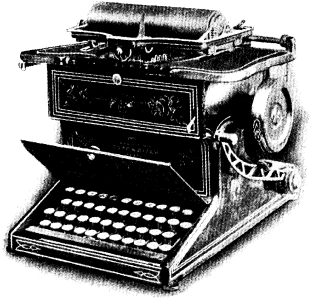
\includegraphics[width=\textwidth]{type_writer2.png}
\end{minipage}

\pause
\vfill

\textit{MRP 2019: Cross-Framework Meaning Representation Parsing}

\begin{minipage}{.6\textwidth}
\begin{itemize}
\item DM, PSD, EDS, UCCA and AMR parsing in English.
\item 18 teams from 8 countries participated.
\end{itemize}
\end{minipage}
\hfill
\begin{minipage}{.1\textwidth}

\includegraphics[width=\textwidth]{logo.png}
\end{minipage}

\pause
\vfill

\textit{MRP 2020: Cross-Framework and Cross-Lingual Meaning Representation Parsing}

\begin{minipage}{.6\textwidth}
\begin{itemize}
\item EDS, PTG, UCCA, AMR and DRG parsing in English, Czech, German and Chinese.
\item 6 teams participated.
\end{itemize}
\end{minipage}
\hfill
\begin{minipage}{.1\textwidth}

\includegraphics[width=\textwidth]{logo.png}
\end{minipage}
\end{frame}


\begin{frame}

\frametitle{SemEval 2019 Task 1: Cross-lingual Semantic Parsing with UCCA}

        \begin{itemize}
            \item 
                English $\{$in-domain/out-of-domain$\} \times 
                \{$open/closed$\}$
            \item
                German in-domain $\{$open/closed$\}$
            \item
                French \textit{low-resource} (only 15 training sentences)
        \end{itemize}


\vfill
\begin{center}
  \begin{minipage}{.3\textwidth}
\includegraphics[width=\textwidth]{wikipedia.png}\end{minipage}
  \begin{minipage}{.3\textwidth}
\includegraphics[width=\textwidth]{squid.jpg}\end{minipage}
\end{center}
\end{frame}


\begin{frame}
\frametitle{Conversion}
\begin{minipage}{.04\textwidth}
\vspace{4mm}
AMR\\
\vspace{13mm}
SDP\\
\vspace{8mm}
\mbox{CoNLL-U}
\end{minipage}
\begin{minipage}{.44\textwidth}
  \centering
  \scalebox{.6}{
  \begin{tikzpicture}[->,
      every node/.append style={sloped,anchor=south,auto=false,font=\tiny},
      level 1/.style={level distance=14mm,sibling distance=26mm},
      level 2/.style={level distance=13mm},
      level 3/.style={level distance=12mm}]
    \node (ROOT) [draw=black,ellipse] {move-01}
      child {node [draw=black,ellipse] {after}
      {
            child {node (graduation) [draw=black,ellipse] {graduate-01} edge from parent node {op1} }
      } edge from parent node {time} }
      child {node (John) [draw=black,ellipse] {person}
      {
        child {node [draw=black,ellipse] {name}
        {
            child {node [draw=black,ellipse] {"John"} edge from parent node {op1} }
        } edge from parent node {name} }
      } edge from parent node {ARG0} }
      child {node [draw=black,ellipse] {city}
      {
        child {node [draw=black,ellipse] {name}
        {
            child {node [draw=black,ellipse] {"Paris"} edge from parent node {op1} }
        } edge from parent node {name} }
      } edge from parent node {ARG2} }
      ;
      \draw (graduation) to node {ARG0} (John);
  \end{tikzpicture}
  }
  
  \vspace{5mm}
  \scalebox{.6}{
    \begin{dependency}[text only label, label style={above}, font=\small]
    \begin{deptext}[column sep=.8em,ampersand replacement=\^]
    After \^ graduation \^ , \^ John \^ moved \^ to \^ Paris \\
    \end{deptext}
        \depedge{1}{2}{ARG2}
        \depedge{5}{4}{ARG1}
        \depedge[edge end x offset=-2pt]{1}{5}{ARG1}
        \deproot[edge unit distance=3.5ex]{5}{top}
        \depedge[edge start x offset=-1pt, edge end x offset=3pt]{5}{7}{ARG2}
        \depedge[edge end x offset=5pt]{6}{5}{ARG1}
        \depedge{6}{7}{ARG2}
    \end{dependency}
    }
    
  \vspace{5mm}
  \scalebox{.6}{
    \begin{dependency}[text only label, label style={above}, font=\small]
    \begin{deptext}[column sep=.8em,ampersand replacement=\^]
    After \^ graduation \^ , \^ John \^ moved \^ to \^ Paris \\
    \end{deptext}
        \depedge{2}{1}{case}
        \depedge{4}{3}{punct}
        \depedge{5}{4}{nsubj}
        \depedge[edge end x offset=-2pt]{2}{5}{obl}
        \depedge{7}{6}{case}
        \deproot[edge unit distance=2.5ex]{5}{root}
        \depedge{5}{7}{obl}
    \end{dependency}
    }

\end{minipage}
\begin{minipage}{.02\textwidth}
\vspace{7mm}
\Leftrightarrow
\vspace{13mm}
\Leftrightarrow
\vspace{18mm}
\Leftrightarrow
\end{minipage}
\begin{minipage}{.45\textwidth}
  \normalsize
  \centering
  \scalebox{.6}{
  \begin{tikzpicture}[level distance=16mm, ->,
      every node/.append style={sloped,anchor=south,auto=false,font=\scriptsize},
      level 1/.style={sibling distance=28mm},
      level 2/.style={sibling distance=14mm},
      level 3/.style={sibling distance=12mm}]
    \tikzstyle{word} = [font=\rmfamily,color=black]
    \node (ROOT) [word] {moved}
      child {node [word] {After}
      {
            child {node (graduation) [word] {graduation} edge from parent node {op} }
      } edge from parent node {time} }
      child {node (John) [fill=black,circle] {}
      {
        child {node [word] {John} edge from parent node {name} }
      } edge from parent node {ARG0} }
      child {node [fill=black,circle] {}
      {
        child {node [word] {Paris} edge from parent node {name} }
      } edge from parent node {ARG2} }
      ;
      \draw[dashed] (graduation) to node {ARG0} (John);
  \end{tikzpicture}}

  \vspace{5mm}
  \scalebox{.6}{
  \begin{tikzpicture}[level distance=14mm, ->,
      every node/.append style={sloped,anchor=south,auto=false,font=\scriptsize},
      level 1/.style={sibling distance=29mm,level distance=6mm},
      level 2/.style={sibling distance=16mm,level distance=14mm}]
    \tikzstyle{word} = [font=\rmfamily,color=black]
    \node (ROOT) [fill=black,circle] {}
      child {node (after) [fill=black,circle] {}
      {
        child {node [draw=none] {}
        {
          child {node [word] (after_word) {After{\color{white}g}} edge from parent [draw=none]}
        } edge from parent [draw=none] }
        child {node [draw=none] {}
        {
          child {node [word] (graduation) {graduation ,} edge from parent [draw=none]}
        } edge from parent [draw=none] }
      } edge from parent node {root}}
      child {node [draw=none] {}
      {
        child {node (moved) [fill=black,circle] {}
        {
          child {node [word] {\quad{\color{white}g} John} edge from parent node {ARG1}}
          child {node [word] {moved{\color{white}g}} edge from parent node {head}}
        } edge from parent [draw=none] }
      } edge from parent [draw=none] }
      child {node (to) [fill=black,circle] {}
      {
        child {node [draw=none] {}
        {
            child {node [word] (to_word) {to{\color{white}g}} edge from parent [draw=none]}
          } edge from parent [draw=none] }
          child {node [draw=none] {}
        {
          child {node [word] (Paris) {Paris{\color{white}g}} edge from parent [draw=none]}
        } edge from parent [draw=none] }
      } edge from parent node {root}}
      ;
      \draw (ROOT) to node {top} (moved);
      \draw (after) to node {head} (after_word);
      \draw (after) to node {ARG2} (graduation);
      \draw[dashed] (after) to node {ARG1} (moved);
      \draw[dashed] (to) to node {ARG1} (moved);
      \draw (to) to node {head} (to_word);
      \draw (moved) to node {ARG2} (Paris);
      \draw[dashed] (to) to node {ARG2} (Paris);
  \end{tikzpicture}}

  \vspace{5mm}
  \scalebox{.6}{
  \begin{tikzpicture}[level distance=15mm, ->,
      every node/.append style={sloped,anchor=south,auto=false,font=\scriptsize},
      level 1/.style={sibling distance=16mm},
      level 2/.style={sibling distance=12mm}]
    \tikzstyle{word} = [font=\rmfamily,color=black]
    \node (ROOT) [fill=black,circle] {}
      child {node (after) [fill=black,circle] {}
      {
        child {node [word] {After{\color{white}g}\quad\quad} edge from parent node {case}}
        child {node [word] {\quad graduation\quad\quad} edge from parent node {head}}
      } edge from parent node {obl}}
      child {node {}
      {
        child {node [word] (comma) {\quad,{\color{white}g}} edge from parent [draw=none]}
      } edge from parent [draw=none]}
      child {node {}
      {
        child {node [word] (John) {John{\color{white}g}} edge from parent [draw=none]}
      } edge from parent [draw=none]}
      child {node {}
      {
        child {node [word] (moved) {moved{\color{white}g}} edge from parent [draw=none]}
      } edge from parent [draw=none]}
      child {node (to) [fill=black,circle] {}
      {
          child {node [word] {to{\color{white}g}} edge from parent node {case}}
          child {node [word] {Paris{\color{white}g}} edge from parent node {head}}
      } edge from parent node {obl}}
      ;
      \draw (ROOT) to node {punct} (comma);
      \draw (ROOT) to node {nsubj} (John);
      \draw (ROOT) to node {head} (moved);
  \end{tikzpicture}}
\end{minipage}
\end{frame}


\begin{frame}
\frametitle{Evaluation}
\begin{adjustbox}{frame,scale=.75,center}
    \begin{tikzpicture}[level distance=12mm, sibling distance=19mm, ->,
        every circle node/.append style={fill=black},
        edge from parent/.append style={nodes={font=\scriptsize}},
        edge from parent path={(\tikzparentnode.center) -- (\tikzchildnode.north)}]
      \tikzstyle{word} = [font=\rmfamily,color=black]
      \node at (0,.7) {True (human-annotated) graph};
      \node (ROOT) at (0,0) [circle] {}
        child {node (After) [word] {After} edge from parent node[left] {L}}
        child {node (graduation) [circle] {}
        {
          child {node [word] {graduation} edge from parent node[left] {P}}
        } edge from parent node[left] {H} }
        child {node [word] {,} edge from parent node[right] {U}}
        child {node (moved) [circle] {}
        {
          child {node (John) [word] {John} edge from parent node[left] {A}}
          child {node [word] {moved} edge from parent node[left] {P}}
          child {node [circle] {}
          {
            child {node [word] {to} edge from parent node[left] {R}}
            child {node [word] {Paris} edge from parent node[right] {C}}
          } edge from parent node[right] {A} }
        } edge from parent node[right] {H} }
        ;
      \draw[dashed,->] (graduation) to node [auto] {\scriptsize A} (John);
      \node at (10.3,.7) {Automatically predicted graph for the same text};
      \node (ROOT_) at (9,0) [circle] {}
        child {node (After_) [word] {After} edge from parent node[left] {L}}
        child {node (graduation_) [circle] {}
        {
          child[alt=<2>{red}{}] {node [word] {graduation} edge from parent node[left] {S}}
        } edge from parent node[left] {H} }
        child {node [word] {,} edge from parent node[right] {U}}
        child {node (moved) [circle,xshift=3mm,yshift=-7mm] {}
        {
          child {node (John_) [word] {John} edge from parent node[left] {A}}
          child {node [word] {moved} edge from parent node[left] {P}}
          child[alt=<2>{red}{}] {node [word] {to} edge from parent node[left] {F}}
          child[alt=<2>{red}{}] {node (Paris_) [word] {Paris} edge from parent node[right] {A}}
        } edge from parent node[right] {H} }
        ;
      \draw[dashed,->] (graduation_) to node [auto] {\scriptsize A} (John_);
      \draw[bend left,dashed,->,alt=<2>{red}{}] (graduation_) to[in=90] node [auto] {\scriptsize A} (Paris_);
    \end{tikzpicture}
\end{adjustbox}
\vfill

\begin{enumerate}
  \item Match primary edges by terminal yield + label.
  \item Calculate \textbf{precision, recall and F1} scores.
  \item Repeat for remote edges.
\end{enumerate}

\pause
\vfill
\begin{adjustbox}{center}
    \begin{tabular}{c|c|c}
        \multicolumn{3}{l}{Primary} \\
        \textbf{P} & \textbf{R} & \textbf{F1} \\ \hline
        $\frac69=67\%$ & $\frac6{10}=60\%$ & 64\%
    \end{tabular}
    \hspace{1cm}
    \begin{tabular}{c|c|c}
        \multicolumn{3}{l}{Remote} \\
        \textbf{P} & \textbf{R} & \textbf{F1} \\ \hline
        $\frac12=50\%$ & $\frac11=100\%$ & 67\%
    \end{tabular}
\end{adjustbox}
\end{frame}

\begin{frame}
\frametitle{Participating Systems}
 8 groups in total:
 \begin{itemize}
 \item
 {\it MaskParse@Deski\~{n}}  {\small Orange Labs, Aix-Marseille University}
 \item
 {\it HLT@SUDA} { \small  Soochow University}
 \item
 {\it T\"{u}Pa} {\small   University of T\"{u}bingen}
 \item
 {\it UC Davis} {\small   University of California, Davis}
 \item    
 {\it GCN-Sem}  {\small   University of Wolverhampton}
 \item
    {\it CUNY-PekingU} {\small 	 City University of New York, Peking University}
 \item
{\it DANGNT@UIT.VNU-HCM} {\small   University of Information Technology VNU-HCM}
 \item
{\it XLangMo} {\small  Zhejiang University}
\end{itemize}

\end{frame}

\begin{frame}
\frametitle{Leaderboard}
\small
\renewcommand*{\arraystretch}{2.1}
\setlength{\tabcolsep}{2pt}
\begin{tabular}{l|lc|lc|lc|lc}
Track&1st place&&2nd place&&3rd place&&baseline\\
\hline
English-Wiki closed&HLT@SUDA&0.774&baseline&0.728&Davis&0.722&0.728\\
English-Wiki open&HLT@SUDA&0.805&CUNY-PekingU&0.800&T\"{u}Pa&0.735&0.735\\
English-20K closed&HLT@SUDA&0.727&baseline&0.672&CUNY-PekingU&0.669&0.672\\
English-20K open&HLT@SUDA&0.767&CUNY-PekingU&0.739&T\"{u}Pa&0.709&0.684\\
German-20K closed&HLT@SUDA&0.832&CUNY-PekingU&0.797&baseline&0.731&0.731\\
German-20K open&HLT@SUDA&0.849&CUNY-PekingU&0.841&baseline&0.791&0.791\\
French-20K open&CUNY-PekingU&0.796&HLT@SUDA&0.752&XLangMo&0.656&0.487
\end{tabular}
\end{frame}


\begin{frame}
    \begin{figure}
        \centering
        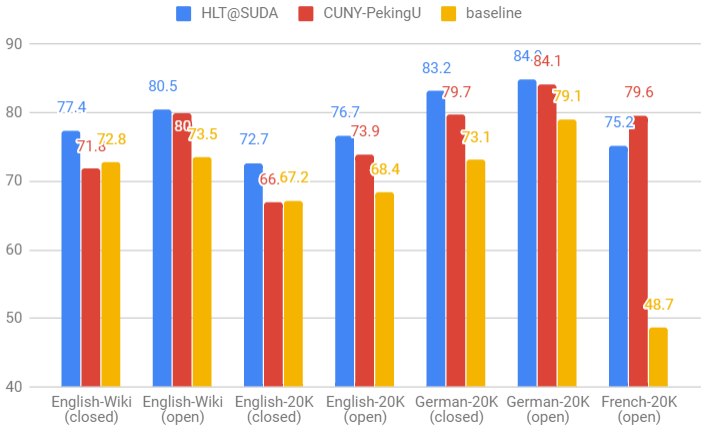
\includegraphics[width=\textwidth]{Capture}
    \end{figure}
\end{frame}



\begin{frame}
\frametitle{Main Findings}

\begin{itemize}
    \item
        HLT@SUDA won 6/7 tracks: \\
        Neural constituency parser + multi-task + BERT \\
        French: trained on all languages, with language embedding
    \pause\item
        CUNY-PekingU won the French (open) track: \\
        TUPA ensemble + synthetic data by machine translation
\end{itemize}
        \pause\vfill
        Surprisingly, results in French were close to English and German
    \begin{itemize}
        \item 
            Demonstrates viability of cross-lingual UCCA parsing
        \item
            Is this because of UCCA's stability in translation?
    \end{itemize}    
\end{frame}


\section{Tasks and Evaluation}

\begin{frame}
\frametitle{What can meaning representation do for NLP?}
 \begin{itemize}
 \item Probing for linguistic knowledge
 \item Querying knowledge bases
 \item \textbf{Underlying explicit structure}
 \end{itemize}
\end{frame}


\begin{frame}
\frametitle{Applications}
\begin{itemize}
  \item Semantics-based evaluation of
  \begin{itemize}
    \item Machine translation \cite{birch2016hume}
    \item Text simplification \cite{sulem2018semantic}
    \item Grammatical error correction \cite{choshen2018reference}
  \end{itemize}
  \item Sentence splitting for text simplification \cite{sulem2018simple}.
\end{itemize}

    \begin{minipage}{0.47\textwidth}
        \centering
        \scalebox{.9}{
                \begin{tikzpicture}[sibling distance=3mm, level distance=7mm,
                every node/.append style={font=\rmfamily},
            	every circle node/.append style={fill=black}]
                \begin{scope}[frontier/.style={distance from root=15mm},
            	edge from parent path={(\tikzparentnode.center) ..
                    controls +(0,-.25) and +(0,.25) .. (\tikzchildnode.north)}]
                \Tree [.\node [circle] (rootu) {};
                \edge node [auto=right]{}; \node (Heu) {He};
                \edge node[auto=right down]{}; \node (gve) {gve};
                \edge node[auto=right]{};
                [.\node [circle](an appleu) {};
                \edge node[auto=right]{}; \node (anu) {an};
                \edge node[auto=left]{}; \node (appleu) {apple};
                ]
                \edge node[auto=left]{};
                [.\node [circle](for john) {};
                \edge node[auto=right]{};\node (for) {for};
                \edge node[auto=left]{}; \node (john) {john};
                ]]
                \end{scope}
                \begin{scope}[yshift=-41mm,grow'=up,
                  frontier/.style={distance from root=12mm},
                  edge from parent path={(\tikzparentnode.center) ..
                  controls +(0,.25) and +(0,-.25) .. (\tikzchildnode.south)}]
                \Tree [.\node [circle] (rootd) {};
                \edge node [auto=left]{}; \node (Hed) {He};
                \edge node[auto=right]{}; \node (gave) {gave};
                \edge node[auto=right]{};\node (John) {John};
                \edge node[auto=right]{};
                [.\node [circle] (an appled) {};
                \edge node[auto=left]{}; \node (and) {an};
                \edge node[auto=right]{}; \node (appled) {apple};
                ]
                ]
                \end{scope}
                \begin{scope}[dashed]
                \draw (Heu) -- (Hed);
                \draw (gve) -- (gave);
                \draw (John) -- (john);
                \draw (anu) -- (and);
                \draw (appleu) -- (appled);
                \end{scope}
                \end{tikzpicture}
        }
    \end{minipage}
    \hspace{1cm}
    \begin{minipage}{0.4\textwidth}
        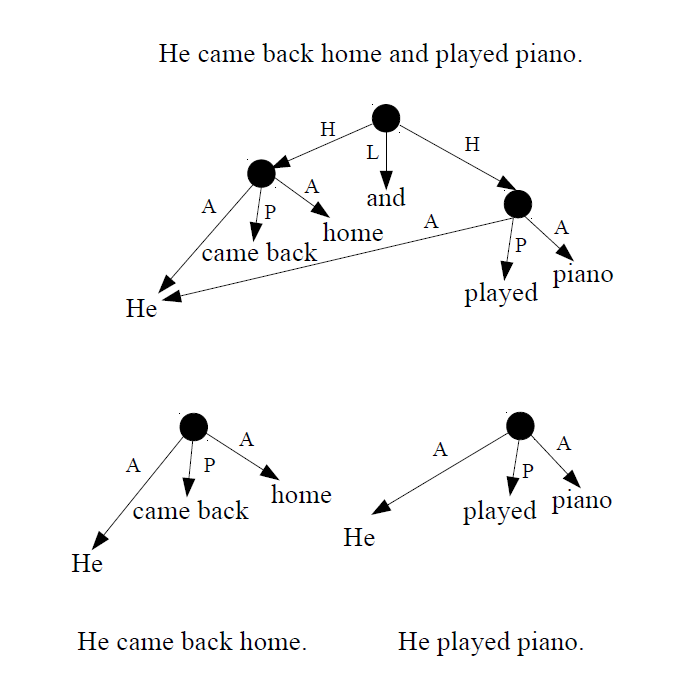
\includegraphics[width=\textwidth,height=48mm]{ucca_simplification}  
    \end{minipage}
\end{frame}

\section{Cross-linguistic Studies}

\frame{\titlepage}

\frame{
\frametitle{References}
\bibliographystyle{acl_natbib}
\bibliography{references}
}


\end{document}
